% mydoc.tex -- my document
% Fred Barnes, March 2014.   <<--- replace with yourself!

\documentclass[a4paper,12pt]{article}
\usepackage{times}
\usepackage{graphicx}

\pagestyle{none}

\begin{document}

\title{Report on Some Stuff}
\author{Fred Barnes \\ frmb@kent.ac.uk}

\date{March 17, 2014}
\maketitle
\begin{abstract}
Abstract
This is an abstract. It can be typeset by using the `abstract' environment
(somewhere between 'maketitle' and the first section usually).You'll also
notice that the typewriter font is slightly different to what you may have 
seen elsewhere. This is done by changing the default typewriter
font in the preamble (see section 2.1).
\end{abstract}


1 Introduction

This is a sample LaTeX document. It includes some bold text, some emphasised
text, plus SOME TEXT TYPESET IN SMALL-CAPS. Small-caps can be selected
in a group by using the `scshape' command, or supplied as an argument to the
`textsc' command.

\textsc{monkey rock}.

1.1 Graphics

One thing that it's useful to be able to do is include graphics or images within
your documents. The common command for this is `includegraphics', whose
main argument is the file-name to get the graphics from (when using pdflatex this
should be a PDF ideally). Various options can be set too, such as scaling of the
graphic. For example:

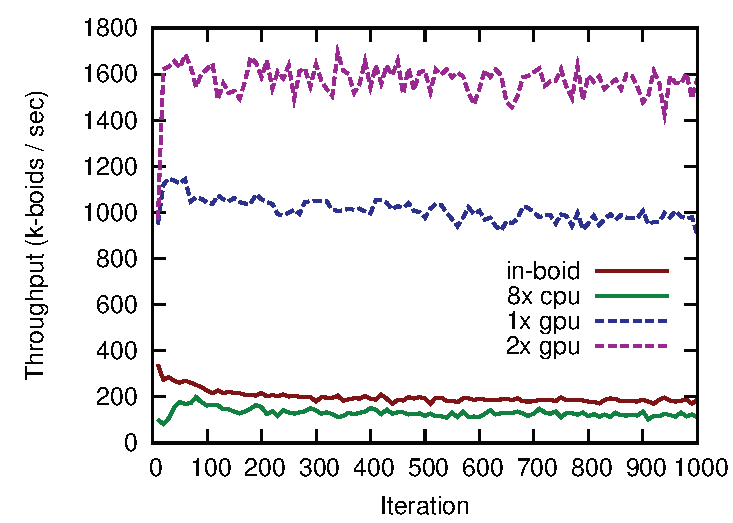
\includegraphics[scale=0.5]{samplegraph1.pdf}

This command comes as part of the `graphicx' package, that must be included using
`usepackage{graphicx}' in the document preamble (else you'll get an error about
an undefined command when running pdflatex).

1.2 Chunks of Verbatim Text

The bit of typewriter text above showing how to use includegraphics is typeset
using the `verbatim' environment. This is slightly special in that all text
(including newlines) are processed as-is, producing a verbatim copy of the input.
This continues until `endcbverbatimcb' is encountered.

2 Results

We ran some tests, and plotted some pretty graphs:

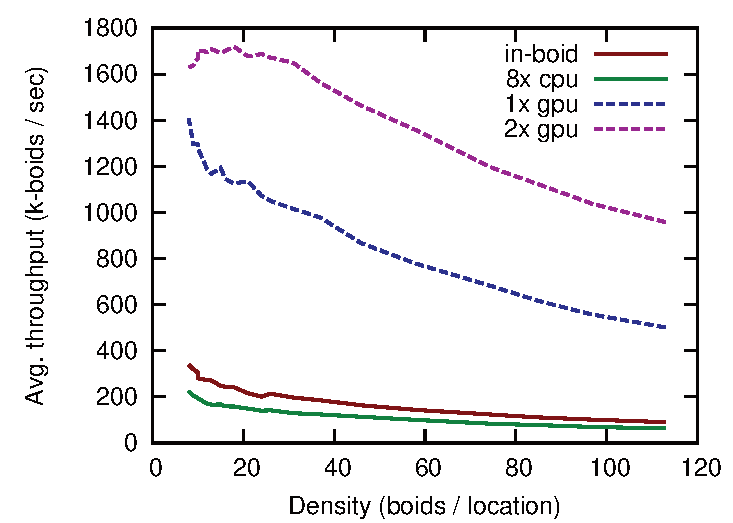
\includegraphics[scale=0.5]{samplegraph2.pdf}

Note: whole graphics (like these) end up being single (and large) boxes for
TEX. As such, they will fall out in the flow of text -- and could be included on a
normal line. The files are `samplegraph1.pdf' and `samplegraph2.pdf'.

2.1 Fixing Your Typewriter
The standard typewriter font isn't very "dense" compared with the selected Times
font. To change this, put the following in the document's preamble:

\renewcommand{\ttdefault}{cmtt}

Closing Remarks

Raptor is a CS unix host. Raptors were also flying dinosaurs that probably lived
on cave-men around at that time (1). Many cave dwelling families probably kept
a tamed pet dinosaur, useful for keeping the rats under control. It's also possible
that cave communities utilised trained homing dinosaurs for exchanging messages
and shipping goods.
\subsection*{This is in an un-numbered sub-section. These can be started using:`subsection*{...}'.}

(1) Some people think that cave-men and dinosaurs didn't exist together, but they weren't there,
so how would they know?



\end{document}
\endinput

